\chapter{Theoretical part}
\label{2-teorie}




\section{Web Processing Services}

The Web Processing Service (WPS) Standard is an OGC standard that provides rules for publishing and executing processes on the web. „The standard also defines how a client can request the execution of a process, and how the output from the process is handled. It defines an interface that facilitates the publishing of geospatial processes and clients’ discovery of and binding to those processes. The data required by the WPS can be delivered across a network or they can be available at the server.“ [1] WPS uses HTTP and XML (eXtensible Markup Language) for describing processes and the data to be exchanged. The first version 0.4.0 was released in 2005 and the current version 2.0 was released in 2015.
A process is essentially a function p that returns an output Y for each input X:\\
\centerline{p: X -> Y}
In case of WPS, a process is a geospatial operation, calculation or a model of any complexity. It may require one or more input arguments and always yields one or more outputs. If there are no input arguments, the process is either generating constant or random values. While WPS was designed for geospatial data, it is not restricted to them.



\begin{figure}[H] \centering
      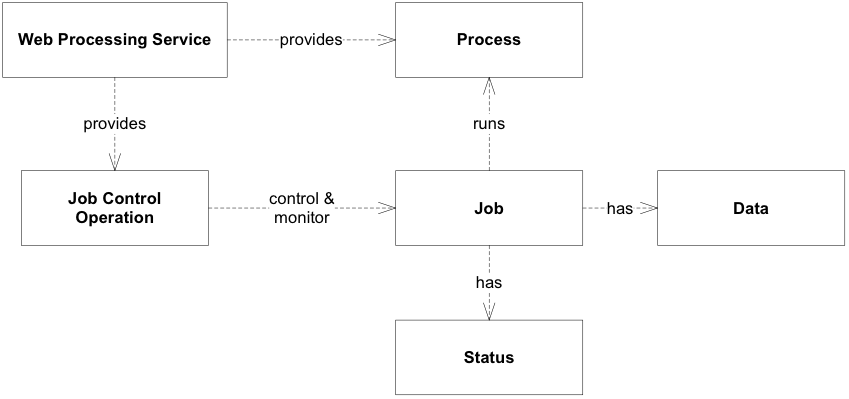
\includegraphics[width=200pt]{./pictures/wps_conceptual_model.png}
      \caption[QGIS logo]{WPS conceptual model (zdroj:
\href{https://www.qgis.org/en/_downloads/qgis-logo.png}{QGIS})}
      \label{fig:qgis}
  \end{figure}


%http://docs.opengeospatial.org/is/14-065/14-065.html#10  link na wps_conceptual_model, hlasi chybu


There are two basic capabilities of a WPS server. It provides the process and retrieves the process description and it controls and monitors processing jobs. Job is an instance of a process – it is an object created for a particular process execution. Job control is the ability to execute, dismiss or delete a job.

\begin{itemize}
\item \textbf{Process execution}
\end{itemize}

There are two ways in which a process can be executed. If the complexity of the process is lower and the completion time is relatively short [3] the execution is run synchronously. After the execute request is sent by the client, the WPS server starts executing the process while the client remains connected to the server for the whole time of the execution process. Only when the process has finished and the output has been delivered, the connection terminates.\par
The asynchronous execution, on the other hand, better suits for complex processes that are expected to take longer time to finish. When the client requests process excecution the server responds with a status information message that confirms the request was accepted and the process will be run. The message also includes a unique processing job identifier. Then, the connection is interrupted. At this time, the client can send the GetStatus request with the job identifier to get information on how the process has progressed. Once the process has finished, the client can access the output data using the GetResult request with the job identifier. The asynchronous execution can be also useful in case of unstable connection that prevents synchronous execution to successfully run.


\subsection{OGC WPS Implementations}





\begin{itemize}
\item \textbf{PyWPS}
	
  
	
\item \textbf{52°North WPS}
	
  

\item \textbf{ZOO Project}
	
\end{itemize}
  


\subsection{ESRI Web Processing}

\section{Geodatabases}

\begin{itemize}
\item \textbf{PostGIS}
	
\item \textbf{Oracle Spatial and Graph}
%Oracle Spatial and Graph, formerly Oracle Spatial
	
\item \textbf{SpatiaLite}

\item \textbf{ArcSDE Geodatabase (ESRI)}
	
\end{itemize}